% DO NOT COMPILE THIS FILE DIRECTLY!
% This is included by the other .tex files.

%\colorlet{punct}{red!60!black}
%\definecolor{background}{HTML}{EEEEEE}
%\definecolor{delim}{RGB}{20,105,176}
%\colorlet{numb}{magenta!60!black}

\lstdefinelanguage{json}{
    basicstyle=\ttfamily\footnotesize,
    numbers=left,
    numberstyle=\ttfamily\footnotesize,
    stepnumber=1,
    numbersep=8pt,
    showstringspaces=false,
    breaklines=true,
    frame=lines,
    backgroundcolor=\color{background},
    literate=
     *{0}{{{\color{numb}0}}}{1}
      {1}{{{\color{numb}1}}}{1}
      {2}{{{\color{numb}2}}}{1}
      {3}{{{\color{numb}3}}}{1}
      {4}{{{\color{numb}4}}}{1}
      {5}{{{\color{numb}5}}}{1}
      {6}{{{\color{numb}6}}}{1}
      {7}{{{\color{numb}7}}}{1}
      {8}{{{\color{numb}8}}}{1}
      {9}{{{\color{numb}9}}}{1}
      {:}{{{\color{punct}{:}}}}{1}
      {,}{{{\color{punct}{,}}}}{1}
      {\{}{{{\color{delim}{\{}}}}{1}
      {\}}{{{\color{delim}{\}}}}}{1}
      {[}{{{\color{delim}{[}}}}{1}
      {]}{{{\color{delim}{]}}}}{1},
}

\begin{frame}[t,plain]
\titlepage
\end{frame}

\begin{frame}
    \frametitle{MISP - VM}
    \begin{itemize}
    \item Credentials
        \begin{itemize}
            \item MISP admin: admin@admin.test/admin
            \item SSH: misp/Password1234
        \end{itemize}
    \item Available at the following location (VirtualBox and VMWare):
        \begin{itemize}
                \item \url{https://www.circl.lu/misp-images/latest/}
        \end{itemize}
    \end{itemize}
\end{frame}

\begin{frame}
    \frametitle{MISP - VM}
    \begin{itemize}
    \item It is a bit broken.
        \begin{itemize}
            \item sudo -s
            \item cd /var/www/MISP/
            \item sudo pear install INSTALL/dependencies/Console\_CommandLine/package.xml
            \item sudo pear install INSTALL/dependencies/Crypt\_GPG/package.xml
            \item cd /usr/local/src/misp-modules
            \item pip3 install -r REQUIREMENTS
            \item pip3 install .
            \item reboot
        \end{itemize}
    \end{itemize}
\end{frame}

\begin{frame}
    \frametitle{MISP - General Usage}
    Plan for this part of the training
        \begin{itemize}
            \item Data model
            \item Viewing data
            \item Creating data
            \item Co-operation
            \item Distribution
            \item Exports
        \end{itemize}
\end{frame}

\begin{frame}
    \frametitle{MISP - Event (MISP's basic building block)}
    \includegraphics[scale=0.45]{screenshots/datamodel1.png}
\end{frame}

\begin{frame}
    \frametitle{MISP - Event (Attributes, giving meaning to events)}
    \includegraphics[scale=0.45]{screenshots/datamodel2.png}
\end{frame}

\begin{frame}
    \frametitle{MISP - Event (Correlations on similar attributes)}
    \includegraphics[scale=0.45]{screenshots/datamodel3.png}
\end{frame}

\begin{frame}
    \frametitle{MISP - Event (Proposals)}
    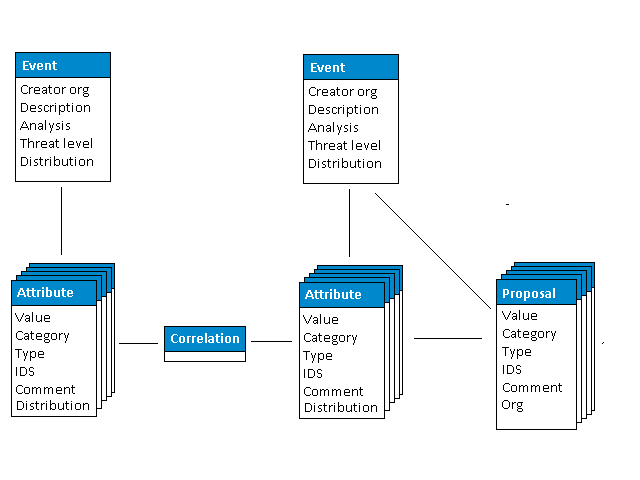
\includegraphics[scale=0.45]{screenshots/datamodel4.png}
\end{frame}

\begin{frame}
    \frametitle{MISP - Event (Tags)}
    \includegraphics[scale=0.45]{screenshots/datamodel5.png}
\end{frame}

\begin{frame}
    \frametitle{MISP - Event (Discussions)}
    \includegraphics[scale=0.45]{screenshots/datamodel6.png}
\end{frame}

\begin{frame}
    \frametitle{MISP - Event (Taxonomies and proposal correlations)}
    \includegraphics[scale=0.35]{screenshots/datamodel7.png}
\end{frame}

\begin{frame}
    \frametitle{MISP - Event (The state of the art MISP datamodel)}
    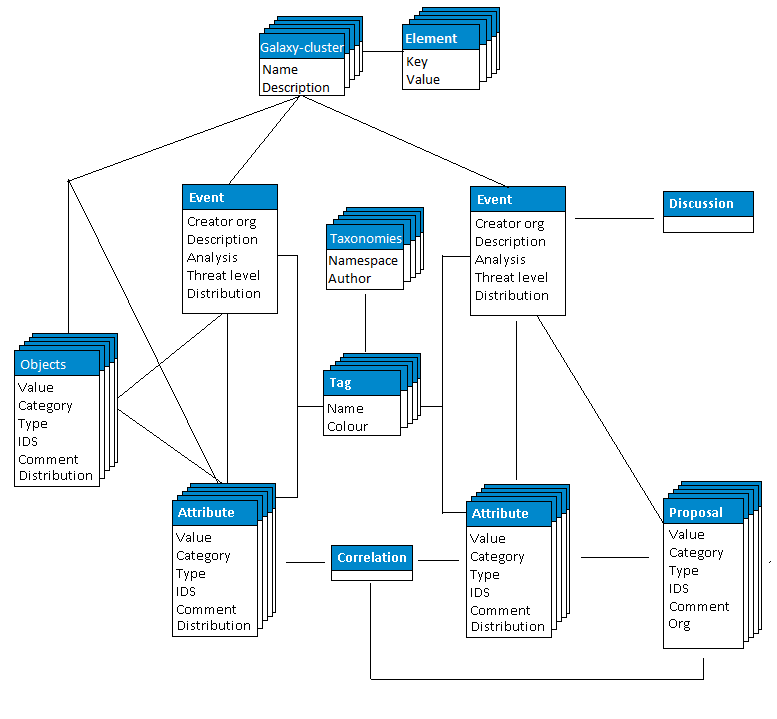
\includegraphics[scale=0.25]{screenshots/datamodel8.png}
\end{frame}

\begin{frame}
    \frametitle{MISP - Viewing the Event Index}
    \begin{itemize}
    \item Event Index
        \begin{itemize}
            \item Event context
            \item Tags
            \item Distribution
            \item Correlations
        \end{itemize}
    \item Filters
    \end{itemize}
\end{frame}

\begin{frame}
    \frametitle{MISP - Viewing an Event}
    \begin{itemize}
     \item Event View
        \begin{itemize}
            \item Event context
            \item Attributes
            \begin{itemize}
                \item Category/type, IDS, Correlations
            \end{itemize}
            \item Objects
            \item Galaxies
            \item Proposals
            \item Discussions
        \end{itemize}
    \item Tools to find what you are looking for
    \item Correlation graphs
    \end{itemize}
\end{frame}

\begin{frame}
    \frametitle{MISP - Creating and populating events in various ways (demo)}
    \begin{itemize}
    \item The main tools to populate an event
        \begin{itemize}
            \item Adding attributes / batch add
            \item Adding objects and how the object templates work
            \item Freetext import
            \item Import
            \item Templates
            \item Adding attachments / screenshots
            \item API
        \end{itemize}
    \end{itemize}
\end{frame}

\begin{frame}
    \frametitle{MISP - Various features while adding data}
    \begin{itemize}
        \item What happens automatically when adding data?
        \begin{itemize}
            \item Automatic correlation
            \item Input modification via validation and filters (regex)
            \item Tagging / Galaxy Clusters
        \end{itemize}
        \item Various ways to publish data
        \begin{itemize}
            \item Publish with/without e-mail
            \item Publishing via the API
            \item Delegation
        \end{itemize}
    \end{itemize}
\end{frame}

\begin{frame}
    \frametitle{MISP - Using the data}
    \begin{itemize}
        \item Correlation graphs
        \item Downloading the data in various formats
        \item API (explained later)
        \item Collaborating with users (proposals, discussions, emails)
    \end{itemize}
\end{frame}

\begin{frame}
    \frametitle{MISP - Sync explained (if no admin training)}
    \begin{itemize}
        \item Sync connections
        \item Pull/push model
        \item Previewing instances
        \item Filtering the sync
        \item Connection test tool
        \item Cherry pick mode
    \end{itemize}
\end{frame}

\begin{frame}
    \frametitle{MISP - Feeds explained (if no admin training)}
    \begin{itemize}
        \item Feed types (MISP, Freetext, CSV)
        \item Adding/editing feeds
        \item Previewing feeds
        \item Local vs Network feeds
    \end{itemize}
\end{frame}

\begin{frame}
    \frametitle{MISP - Distributions explained}
    \begin{itemize}
        \item Your Organisation Only
        \item This Community Only
        \item Connected Communities
        \item All Communities
        \item Sharing Group
    \end{itemize}
\end{frame}

\begin{frame}
    \frametitle{MISP - Distribution and Topology}
    \includegraphics[scale=0.45]{screenshots/sync.png}
\end{frame}

\begin{frame}
    \frametitle{MISP - Exports and API}
    \begin{itemize}
        \item Download an event
        \item Quick glance at the APIs
        \item Download search results
        \item ReST API and query builder
    \end{itemize}
\end{frame}

\begin{frame}
    \frametitle{MISP - Shorthand admin (if no admin training)}
    \begin{itemize}
        \item Settings
        \item Troubleshooting
        \item Workers
        \item Logs
    \end{itemize}
\end{frame}
